\subsection{Main Game Loop}
	 The Main Game Loop is the contains the main function in which all game logic is performed. The game logic is performed using the classes described above. The following class diagram, figure \ref{fig:classMain}, shows the dependencies for the Main Game Loop. 

	\begin{figure}[H]
		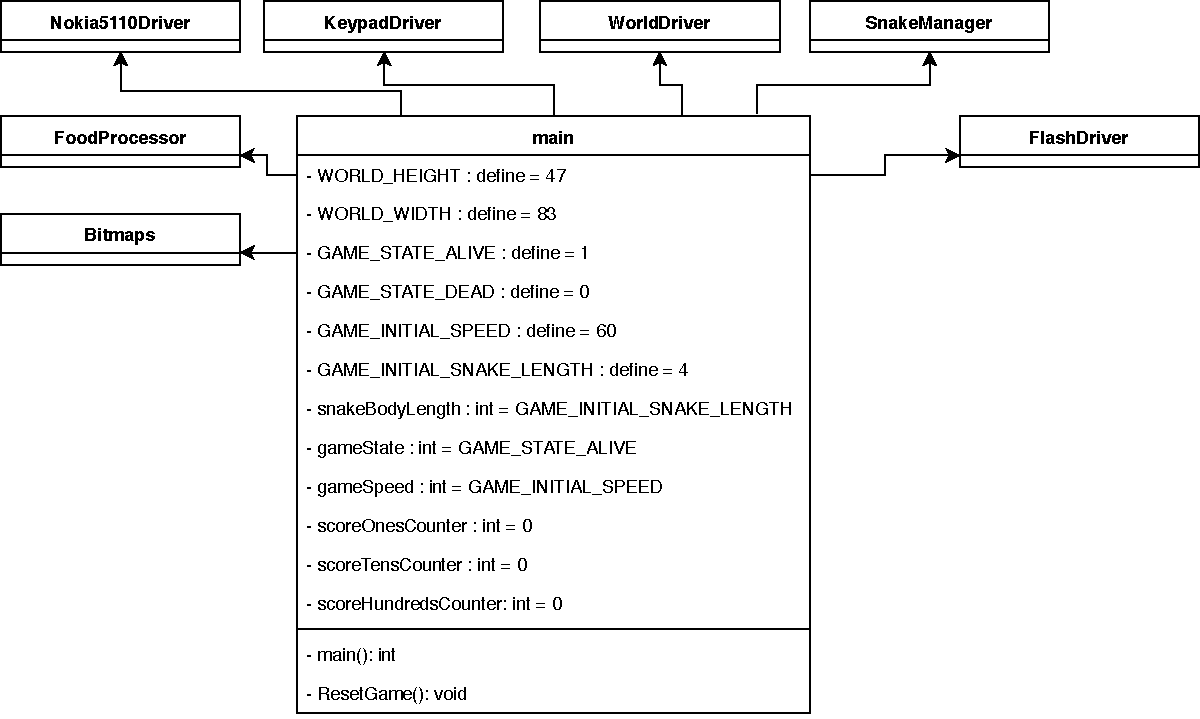
\includegraphics[width=14cm]{MainClassDiagram}
		\centering
		\caption{Class diagram for MainGameLoop}
		\label{fig:classMain}
	\end{figure}
	

\begin{table}[H]
	\centering
	\begin{tabular}{|l|l|}
		\hline
		\multicolumn{1}{|c|}{\textbf{Attribute}} & \multicolumn{1}{c|}{\textbf{Description}} \\ \hline
		\begin{tabular}[c]{@{}l@{}}WORLD\_HEIGHT/\\ WORLD\_WIDTH\end{tabular} & \begin{tabular}[c]{@{}l@{}}These attributes describe the pixel dimensions for the \\Nokia 5110 Display.\end{tabular} \\ \hline
		\begin{tabular}[c]{@{}l@{}}GAME\_STATE\_ALIVE/\\ GAME\_STATE\_DEAD\end{tabular} & These attributes describe the gamestate. \\ \hline
		\begin{tabular}[c]{@{}l@{}}GAME\_INITAL\_SPEED/\\ GAME\_INITIAL\_\\ SNAKE\_LENGTH\end{tabular} & \begin{tabular}[c]{@{}l@{}}These attributes describe inital values for the frame\\ rate of the display and for the length \\of the snake. When the game is reset the speed and \\length are reset to these values.\end{tabular} \\ \hline
		snakeBodyLength & \begin{tabular}[c]{@{}l@{}}Indicates the current length of the snake. This value\\ is incremented twice each time the snake collides with\\ food.\end{tabular} \\ \hline
		gameState & \begin{tabular}[c]{@{}l@{}}Indicates the current game state. This is used to \\determine if the game should be reset and if the high\\ score should be displayed.\end{tabular} \\ \hline
		gameSpeed & \begin{tabular}[c]{@{}l@{}}Indicates the frame rate of the display. This value\\ translates to the speed of the snake movement.\end{tabular} \\ \hline
		\begin{tabular}[c]{@{}l@{}}scoreOnesCounter/\\ scoreTensCounter/\\ scoreHundredsCounter\end{tabular} & \begin{tabular}[c]{@{}l@{}}Indicates the score which combined make up a three\\ digit score. The hundreds counter is not displayed and\\ is used to roll over the score if it exceeds 99.\end{tabular} \\ \hline
	\end{tabular}
	\caption{Description of the attributes of MainGameLoop}
	\label{my-label}
\end{table}

-- Hit detection
-- World rendering
-- Reset logic
-- Highscore



